\section{Introduction}

%\begin{figure}[t]
%	\centering
%	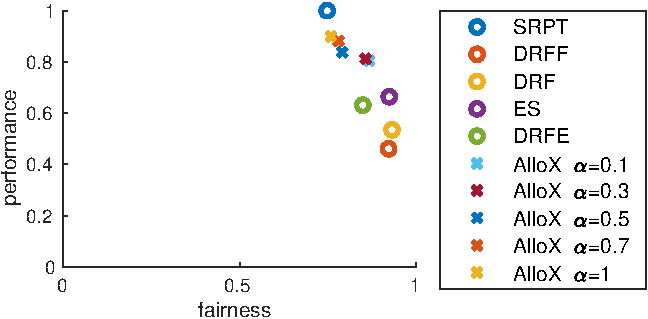
\includegraphics[width=1.0\linewidth]{figs/perf_fair_tradeoffs}
%	\caption{\name improves the performance of average completion time by up to 35\% while maintains fairness level closely to the traditional fair schedulers.}
%	\label{fig:motivation}
%\end{figure}

\desc{Background: rapid growth of machine learning applications, CPU/GPU cluster, ML jobs and other jobs share the same cluster}

In modern computer systems, multiple resources can be used in an interchangeable way to fulfill the same demand. 
In particular, CPUs and (GP)GPUs can be used for the computation in job processing \cite{tensorflow, debunking, coordinating-gpu-cpu, fpga-gpu-cpu}. 
Generally speaking, CPUs are more efficient for complicated computations with a limited number of threads running in parallel. A powerful server nowadays normally has tens of CPU cores~\cite{intel-xeon}. 
In contrast, GPUs are used primarily for highly parallelized yet simple computations. A single GPU can have as many as 5,120 cores~\cite{nvidia-volta}, each of which runs at a lower frequency and supports limited operations. Recently, GPUs are becoming popular for deep learning, massive data mining, and even networking \cite{fpga-gpu-cpu, tensorflow, packetshader}. Noticeably, Google has developed a specialized FPGA-based processor named TPU for its AI system AlphaGo~\cite{tpu}. 
It is common to run jobs on a cluster consisted of interchangeable resources. 

% All these resources, however, are used by multiple users, potentially from different entities, and they share the same physical infrastructure. 
% Examples of such shared environments include Amazon EC2, Microsoft Azure, and Google Compute \cite{ec2, azure, google-compute} as well as private clusters. 
% The system needs to first allocate resources to these users, while satisfying some basic properties, such as sharing incentive (SI), Pareto efficiency (PE), and strategyproofness (SP) \cite{drf}. After receiving the resources, each user can decide how to run her jobs, e.g., first come first served or shortest remaining processing time first~\cite{sjf}.

\desc{Single configuration vs multiple configurations} 

In such clusters, jobs have more than one configurations. 
Traditionally, a job only has the CPU configuration. For instance, if a job needs 1 CPU and 12 GB Memory (MEM), its CPU configuration is (1 CPU, 12GB MEM). 
With the recent progress on machine learning frameworks such like Tensorflow~\cite{tensorflow}, a wide variety of jobs can be executed on both CPUs and GPUs. 
In addition to the CPU configuration, a job has another GPU configuration, such as (1 GPU, 2GB MEM). 
In the state-of-the-art systems, such as Kubernetes~\cite{kubernetes} for containerized applications, users need to specify either the CPU configuration or the GPU one before a job can be processed. 
The job processing time varies a lot under CPU or GPU configurations. 
In Section~\ref{sec:speedup}, we present experimental results to show that different jobs have distinct speedup using GPUs compared to CPUs .

%so it can have 2 configurations: CPU and GPU configurations.
%For example, a job needs <20 CPU cores, 12 GB RAM> or <1 GPU, 2GB RAM>.

%In \name, the system is shared by multiple users, and each user has a sequence of jobs. In some existing work, there are multiple jobs, each consisted of multiple tasks. The similarity is by scheduling and placement of jobs in \name (or tasks in other systems) to optimize performance and fairness for users (or jobs in other systems). 

\desc{Problem: how to effectively schedule different types of jobs}

The \emph{central problem} of this paper is \emph{how to pick the configuration for each job and order the jobs} to optimize performance objectives such as average job completion time while providing fair resource allocations among multiple users. This needs to be done in an online manner with minimal efforts from users.

% \emph{Problem statement.} The goal of \name is to automatically estimate job demand and schedule jobs to maximize performance objectives while providing fair allocations among users. The resource manager for multiple configuration jobs must pick (i) the configuration to use for each job and 
% (ii) the order and placement of jobs to optimize performance and fairness objectives. 

%\zhenhua{I edited the description of the example, but we need an example with a better improvement.}
Consider a simple example in Table \ref{tbl:mov_example}, where two users share a small cluster of two CPUs and two GPUs. 
Each user has 3 jobs queued up at the beginning that can be processed on either CPUs or GPUs with the processing times shown in the last two columns.
% Each job can execute either on CPU or GPU with different completion times.
% The GPU/CPU speed-up rates of jobs are different.
%6 jobs are queued up at the beginning.

% \begin{table}[H]    
% 	\caption{A motivating example.\todo{relabel the job ID and redraw figure 1 in the same style of other figures in the paper.}}
% 	\label{tbl:mov_example}
% 	\begin{tabular}{|c|c|c|c|}
% 		\hline
% 		User & Job ID & Compl. on GPU & Compl. on CPU \\  \hline \hline
% 		User 1 & 1 & 3 & 4 \\  \hline
% 		User 1 & 3 & 1.5 & 4 \\  \hline
%         User 1 & 5 & 1 & 2 \\  \hline
% 		User 2 & 2 & 3 & 3 \\  \hline
%         User 2 & 4 & 2 & 3 \\  \hline		
% 		User 2 & 6 & 1.5 & 2 \\  \hline
% 	\end{tabular}
% \end{table}

% \xiao{I made a new example as below}
\begin{table}[t]
	\caption{A motivating example. PT stands for processing time in minutes. }\vspace{-0.1in}
	\label{tbl:mov_example}
	\begin{tabular}{|c|c|c|c|}
		\hline
		User & Job ID & PT on GPU & PT on CPU \\  \hline \hline
		User 1 & 1 & 10 & 15 \\  \hline
		User 2 & 2 & 8 & 10 \\  \hline
        User 1 & 3 & 10 & 50 \\  \hline
		User 2 & $  $4 & 5 & 75 \\  \hline
        User 1 & 5 & 10 & 15 \\  \hline		
		User 2 & 6 & 10 & 15 \\  \hline
	\end{tabular}\vspace{-0.2in}
\end{table}


\begin{figure}[!htbp]
	\centering
	{
\includegraphics[width=0.45\linewidth]{figs/example_legend} }    \hspace{0.0in} \\
	\subfloat[Equal Share] {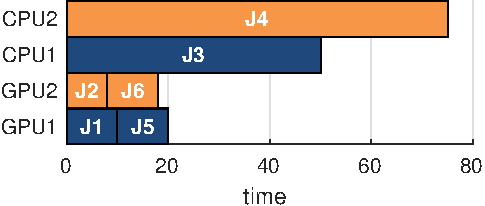
\includegraphics[width=0.7\linewidth]{figs/example_fair} \label{fig:motivation_example_1}}\vspace{-0.1in}    \hspace{-0.1in}
	\subfloat[\name] {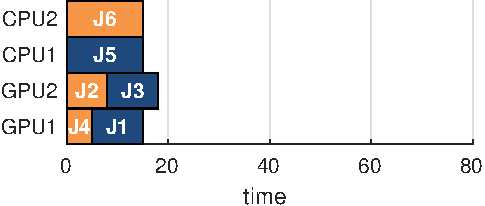
\includegraphics[width=0.7\linewidth]{figs/example_opt} \label{fig:motivation_example_2}}   \vspace{-0.1in} \hspace{-0.1in}		\caption{Improvement from \name scheduling.
}\vspace{-0.2in}
	\label{fig:motivation_example}
\end{figure}

%\xiao{The numbers are $\frac{181}{6}$ vs $\frac{76}{6}$, with around 59\% improvement}

Figure \ref{fig:motivation_example} compares a strawman solution and our solution \name developed in this paper.
The strawman solution in Figure \eqref{fig:motivation_example_1} divides CPUs and GPUs equally between the two users and places the jobs on CPUs and GPUs in a First-Come-First-Served (FCFS) manner. 
When it is the turn for a particular job to run, this job picks its ``favorite'' resource (the one results in shorter processing time) if that resource is available, otherwise it picks the other resource. This equal sharing solution results in an average job completion time of $\frac{181}{6}$ minutes.

%~\todo{How to pick the configuration? What's FCFS given jobs are queued at the beginning?}.  \xiao{To be specific, for each user, we consider the job in order based on the job ID, and we place the job to its favorite device - unless that device is full and there is another device available for that user to schedule the job. For example, for job 3, its favorite device is GPU, but GPU is already full as GPU is being used by job 1, so it has to take CPU}


%The strawman solution fully utilizes the resources but its performance is far from optimal.
Figure \eqref{fig:motivation_example_2} illustrates our solution, which is significantly better.
The average job completion time is reduced to $\frac{76}{6}$ minutes, a $59\%$ improvement. The makespan is also reduced by $76\%$. 


\desc{Motivating example: why interchangeability makes the problem more challenging? (i) average job completion time: SRPT => NP-hard; (ii) resource utilization: work conservation is not good enough; (iii) fairness: DRF is no longer optimal.}

While the improvement is huge, there are significant algorithmic and systems challenges with multiple job configurations. From the performance's perspective, while minimizing the average job completion time is relatively easy when jobs have only one configuration \cite{labetoulle1984preemptive}, the problem is APX-hard when there are multiple configurations by a reduction from a maximum bounded 3-dimensional matching problem \cite{hoogeveen1998non}. %even if we only have two configurations. The proof is from the reduction of \todo{add details}\xiao{look for proving $Rm|pmtn|\sum C_j$ is NP-hard}. When there are arrivals over time, even if the arrival time is known to the scheduler beforehand, the problem becomes APX-hard when there are multiple configurations \todo{add one sentence explanation or point to later section where you have detailed explanations.}. The reduction comes from a maximum bounded 3-dimensional matching problem \cite{hoogeveen1998non}.
%
% ~\todo{Xiao, do you have a detailed explanations?}
% \todo{Show that multiple configurations makes the problem hard }
%
% For example, where there is only one configuration, meaning that only 1 type of resource will be used for computation, the problem is polynomially solvable when all jobs start at the beginning and preemption is allowed, policies like SRPT can tackle these secenarios easily. However, when multiple configurations are allowed, the problem becomes strongly NP-Hard \cite{sitters2001two}, 
% and when there are arrivals - even offline arrivals, meaning that the scheduler knows the arrival times of all jobs, the problem becomes APX-Hard \cite{hoogeveen1998non}.
%
% when there are more than one configurations. For example, for single machine or parallel and identical machine, when all jobs arrives over time, minimizing the average job completion time is relatively easy when each job only has one configuration \cite{afrati1999approximation}. When there are more than one configurations, the problem is equivalent to online scheduling with unrelated machines, where each machine can be viewed as an individual CPU or GPU resource. This problem is APX-Hard \cite{hoogeveen1998non}, even when preemption is allowed. The hardness can be obtained from a Maximum Bounded 3-dimensional matching problem.
%
Regarding fairness, while the Dominant Resource Fairness (DRF) allocation and its variants
~\cite{drf,hug,parkes2015beyond, drfq,choosy,drf_hetor} provide desirable properties, there exists a hard tradeoff among the fundamental properties with multiple job configurations and DRF fails to provide most properties. %That partially explains why strawman solutions in Figure~\ref{fig:motivation_example_1} and later in Section~\ref{sec:perf-strawman} do not work well. 
For system development, existing systems heavily rely on users to provide key information such as which configuration to use in Kubernetes while users may not have the expertise or the system-level information to do so.

We make the following contributions in tackling these challenges by designing \name. 

\begin{itemize}
\item Motivated by experimental results on a real system, we identify a new job scheduling and resource allocation problem and analyze the inefficiencies of existing solutions (\S\ref{sec:background}). Specifically, most existing solutions may lead to \emph{arbitrarily} poor performance when jobs have multiple configurations. %, and the widely used DRF allocation fails to provide most desirable properties . 
\item We design the \name algorithm to optimize performance and provide dynamic fair allocation (\S\ref{sec:alg}). Our key idea is to transform the multi-configuration job scheduling problem into a min-cost bipartite matching problem, which can be solved in polynomial time. It provides the optimal solution in simplified settings and outperforms all baselines significantly in general settings. \name dynamically schedules jobs from the users with the lowest progress for fairness.
%We discuss the new implications of the properties in {\name} and show that it is impossible to achieve SI, SP, and PE simultaneously in \name in \S\ref{sec:fairness}.
\item We implement \name on Kubernetes (\S\ref{sec:system}). Besides the scheduling algorithm, \name profiles jobs in an online manner to automatically decide job configurations and estimates job processing times under different configurations. Both are necessary inputs for the scheduling algorithm. 
\item We conduct experimental and numeric evaluations to show the performance improvements (\S\ref{sec:evaluation}). Results highlight that \name reduces the average job completion time significantly, provides good fairness among users, and prevents starvation.
\end{itemize}


% Our key idea is to transform the multi-configuration job scheduling problem into a network flow problem


% \begin{figure}[t]
% 	\centering
% 	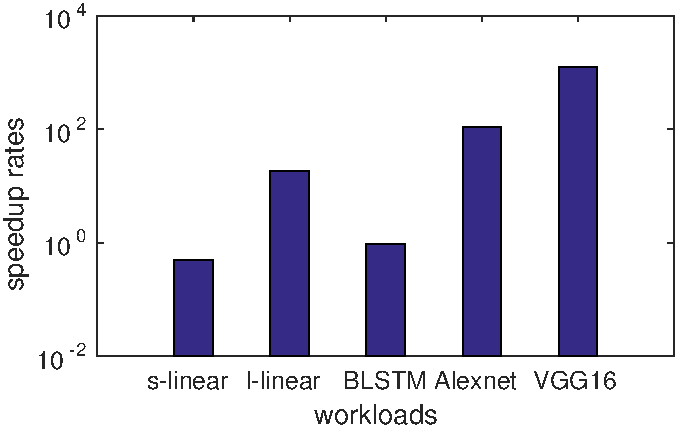
\includegraphics[width=0.7\linewidth]{figs/beta}
% 	\caption{Jobs have different speed-up rates when running on GPUs.}
% 	\label{fig:beta}
% \end{figure}

% % In this paper, we consider the interchangeable resource allocation (\name) problem to decide how to allocate interchangeable resources to multiple users while satisfying the desired properties.  
% % In the new {\name} problem, traditional multi-resource allocation policies such as DRF~\cite{drf} and its variants~\cite{beyond-drf, choosy, hdrf, hug} do not work. In particular, we show that a straightforward application of DRF to \name fails to provide SI, SP, or PE properties. 



% This paper is the first step towards understanding and analyzing this general case. We aim to answer the following questions: (i) Is it possible in {\name} to provide those properties satisfied in the traditional multi-resource allocations? (ii) Can we design efficient algorithms to achieve (or approximate if (i) is impossible) these properties? (iii) How much performance improvements can these algorithms get?




% \desc{Opportunity: CPU low utilization (forward pointing to later figure), identify job types and place jobs on CPU or GPU accordingly}

% Existing systems such as Kubernetes ask users to decide job demand and where to place the job, CPU or GPU~\cite{yarn, kubernetes, mesos}, to simplify the design of schedulers. However, users may not have enough expertise or information to make such choices, leading to significant inefficiencies as shown in Section~\ref{sec:background}. 
% When we allow users to choose the configurations to run their jobs in hybrid CPU/GPU clusters, it may easily result in one of resource become the bottleneck.
% When most people think GPUs are the better resources for them, GPUs can be overloaded while CPUs are abundant and mostly under-utilized like Figure \ref{fig:avg_util}.

% \desc{Our idea: periodic scheduling for fairness, network algorithm for multiple configurations, online profiling for information (explain the importance of having the information)}

% The key motivation for this work is that different users and applications may have dramatically different efficiencies in utilizing GPU for computation.
% Figure~\ref{fig:beta} illustrates results from real experiments.  We start from a simple workload such as linear regression \cite{tensorflow-examples} and consider standard benchmarks such as AlexNet and VGG16 \cite{tensorflow-benchmark}. We consider two linear regression jobs, i.e., s-linear and l-linear, where s-linear has only 200 data points for training and l-linear has 10000 data points. Bidirectional long-short-term memory (BLSTM) is the deep learning architecture that works well with text data ~\cite{deep-learning-cpu-gpu-benchmark}. AlexNet and VGG16 are both well-known convolution neural network (CNN) models. The numbers show how much speedup one GPU (Tesla P100 16GB) can bring compared to only using one physical CPU core (E5-2670 v3 @ 2.30GHz). While GPU is very efficient in accelerating computations (1 GPU can speedup the computation by 1230 times) for applications such as VGG16, AlexNet~\cite{tensorflow-benchmark}, and l-linear~\cite{tensorflow-examples}, it is not very useful for other applications such as s-linear~\cite{tensorflow-examples} and BLSTM~\cite{deep-learning-cpu-gpu-benchmark}.
% We discuss the detailed conversion from GPU to CPU in \S\ref{sec:background}.

% At a high level, we can use a $n\times n$ matrix $\mathbf{E}$ to represent a system of $n$ resources, where the element $e_{ij}$ represents how efficiently resource $i$ can be replaced by resource $j$.
% Then single resource allocation only deals with a $1\times1$ matrix, while the traditional multi-resource allocation extends it to an identity matrix. {\name} works with a general matrix which is not necessarily diagonal. %\todo{add a figure}


%Contributions: (i) identify the problem; (ii) efficient algorithm design; (iii) system implementation and evaluation
